\documentclass[10pt]{beamer}
% \setbeameroption{show only notes}

\usetheme[progressbar=foot]{metropolis}
\makeatletter
\usepackage[caption=false]{subfig}
\usepackage{float}
\usepackage{textgreek}
\newlength\beamerleftmargin
\setlength\beamerleftmargin{\Gm@lmargin}
\usepackage[absolute,overlay]{textpos}
\usepackage{appendixnumberbeamer}
\setbeamertemplate{section in toc}[sections numbered]
\setbeamertemplate{subsection in toc}[subsections numbered]
\usepackage{booktabs}
\usepackage[scale=2]{ccicons}
\definecolor{utred}{RGB}{204,0,0}
\definecolor{utgray}{RGB}{128,128,128}
\usepackage{tikz}
\usepackage{graphicx}
\usepackage{pgfplots}
\usepackage{caption}
\captionsetup[figure]{labelformat=empty}
\setbeamertemplate{subsection in toc}
{\leavevmode\leftskip=2em\rlap{\hskip-2em$\quad$\inserttocsectionnumber.\inserttocsubsectionnumber}$\quad$\inserttocsubsection\par}
%%%%%%
\usepgfplotslibrary{dateplot}

\usepackage{xspace}
\newcommand{\themename}{\textbf{\textsc{metropolis}}\xspace}

\title{Platelet Priming and Rolling}
\date{\today}
\author{Andrew Watson}
\institute{University of Utah}
% \titlegraphic{\hfill\includegraphics[height=1.5cm]{logo.pdf}}

\setbeamercolor{progress bar in head/foot}{fg=utred,bg=utgray}
\setbeamercolor{progress bar in section page}{fg=utred,bg=utgray}
\setbeamercolor{progress bar in title separator}{fg=utgray,bg=black}
\setbeamercolor{frametitle}{bg=utred, fg=white}
\setbeamercolor{block title alerted}{fg=utred}
\setbeamercolor{alerted text}{fg = utred}
\setlength{\metropolis@titleseparator@linewidth}{1.5pt}
\setlength{\metropolis@progressonsectionpage@linewidth}{1.5pt}
\setlength{\metropolis@progressinheadfoot@linewidth}{3pt}
\setlength{\metropolis@progressonsectionpage@linewidth}{1.5pt}

\setbeamerfont{bibliography item}{size=\scriptsize}
\setbeamerfont{bibliography entry author}{size=\scriptsize}
\setbeamerfont{bibliography entry title}{size=\scriptsize}
\setbeamerfont{bibliography entry location}{size=\scriptsize}
\setbeamerfont{bibliography entry note}{size=\scriptsize}

\setlength{\fboxsep}{0pt}
\setlength{\fboxrule}{.25pt}

\newcommand{\vect}[1]{\boldsymbol{\mathbf{#1}}}
\newcommand{\tn}{\textnormal}

\begin{document}

\maketitle

\addtobeamertemplate{frametitle}{}{%
\begin{tikzpicture}[remember picture,overlay]
  \node[anchor=north east,yshift=2pt] at (current page.north east)
  {\includegraphics[height=0.7cm]{ulogo@2x.png}};
\end{tikzpicture}}

\section{Biological Motivation \& Current Project}

\begin{frame}{Summary of rolling biology}
  \begin{itemize}
  \item Platelets are activated by agonists
  \item In injured blood vessels, immobilized agonists are exposed on
    the wall
  \item Inactive platelets transiently bind with agonists on the wall
    $\rightarrow$ slows down \& activates platelet $\rightarrow$ firm
    adhesion \& start of coagulation
  \end{itemize}
\end{frame}

\begin{frame}{Priming experiments}
  \begin{figure}
    \centering
    \setlength{\fboxsep}{0pt}
    \setlength{\fboxrule}{.25pt}
    \fbox{\includegraphics[width=.75\textwidth]{expt-sideview}}
    \caption{Side view of the priming microfluidic
      chambers. Eichinger, Ph.D. dissertation, 2016}
    \label{fig:flow-chambers}
  \end{figure}

  \begin{itemize}
  \item Nonlocal effects---experiments from
    Proteins-Polymers-Interfaces group led by Dr. Hlady
    \note[item] {Brief background: they are generally interested in
    designing materials that can be implanted into bloodstream without
    triggering clotting \& immune responses}
  \item Platelets can transiently bind to agonists without firmly
    adhering, and be primed for full downstream activation
    \note[item] {Perhaps not surprising, but not considered or
    quantified in traditional materials tests}
  \end{itemize}
\end{frame}

\begin{frame}{Priming Experiments}
  \begin{figure}
    \centering
    \fbox{\includegraphics[width=.75\textwidth]{expt-sideview}}
    \caption{Side view of the priming microfluidic
      chambers. Eichinger, Ph.D. dissertation, 2016}
    \label{fig:flow-chambers}
  \end{figure}

  \begin{itemize}
  \item Some results: more primed platelets adhere in the capture
    region than unprimed, primed platelets have higher levels of
    P-selectin expression and active
    \textalpha\textsubscript{IIb}\textbeta\textsubscript{3} 
  \item Rolling data extracted: average velocities, step sizes, pause times
  \end{itemize}
\end{frame}

\begin{frame}{Adhesive dynamics models}
  \note[item] {Rolling specifically refers to the combined physical and
  chemical process of platelet motion in blood near a vessel wall, and
  binding kinetics of platelet receptors with immobilized agonists}
\begin{columns}
  \begin{column}{.5\textwidth}
    \begin{itemize}
    \item Components of Adhesive Dynamics models:
      \begin{itemize}
      \item Random bond formation and breaking (tracking individual
        receptors and bonds)
      \item FSI: Stokes flow around a rigid body (spheres in
        traditional AD, ellipsoids in platelet AD)
      \end{itemize}
    \item Bond-level kinetics $\rightarrow$ cell-level behavior
    \end{itemize}
  \end{column}

  \begin{column}{.5\textwidth}
    \begin{figure}
      \centering
      \fbox{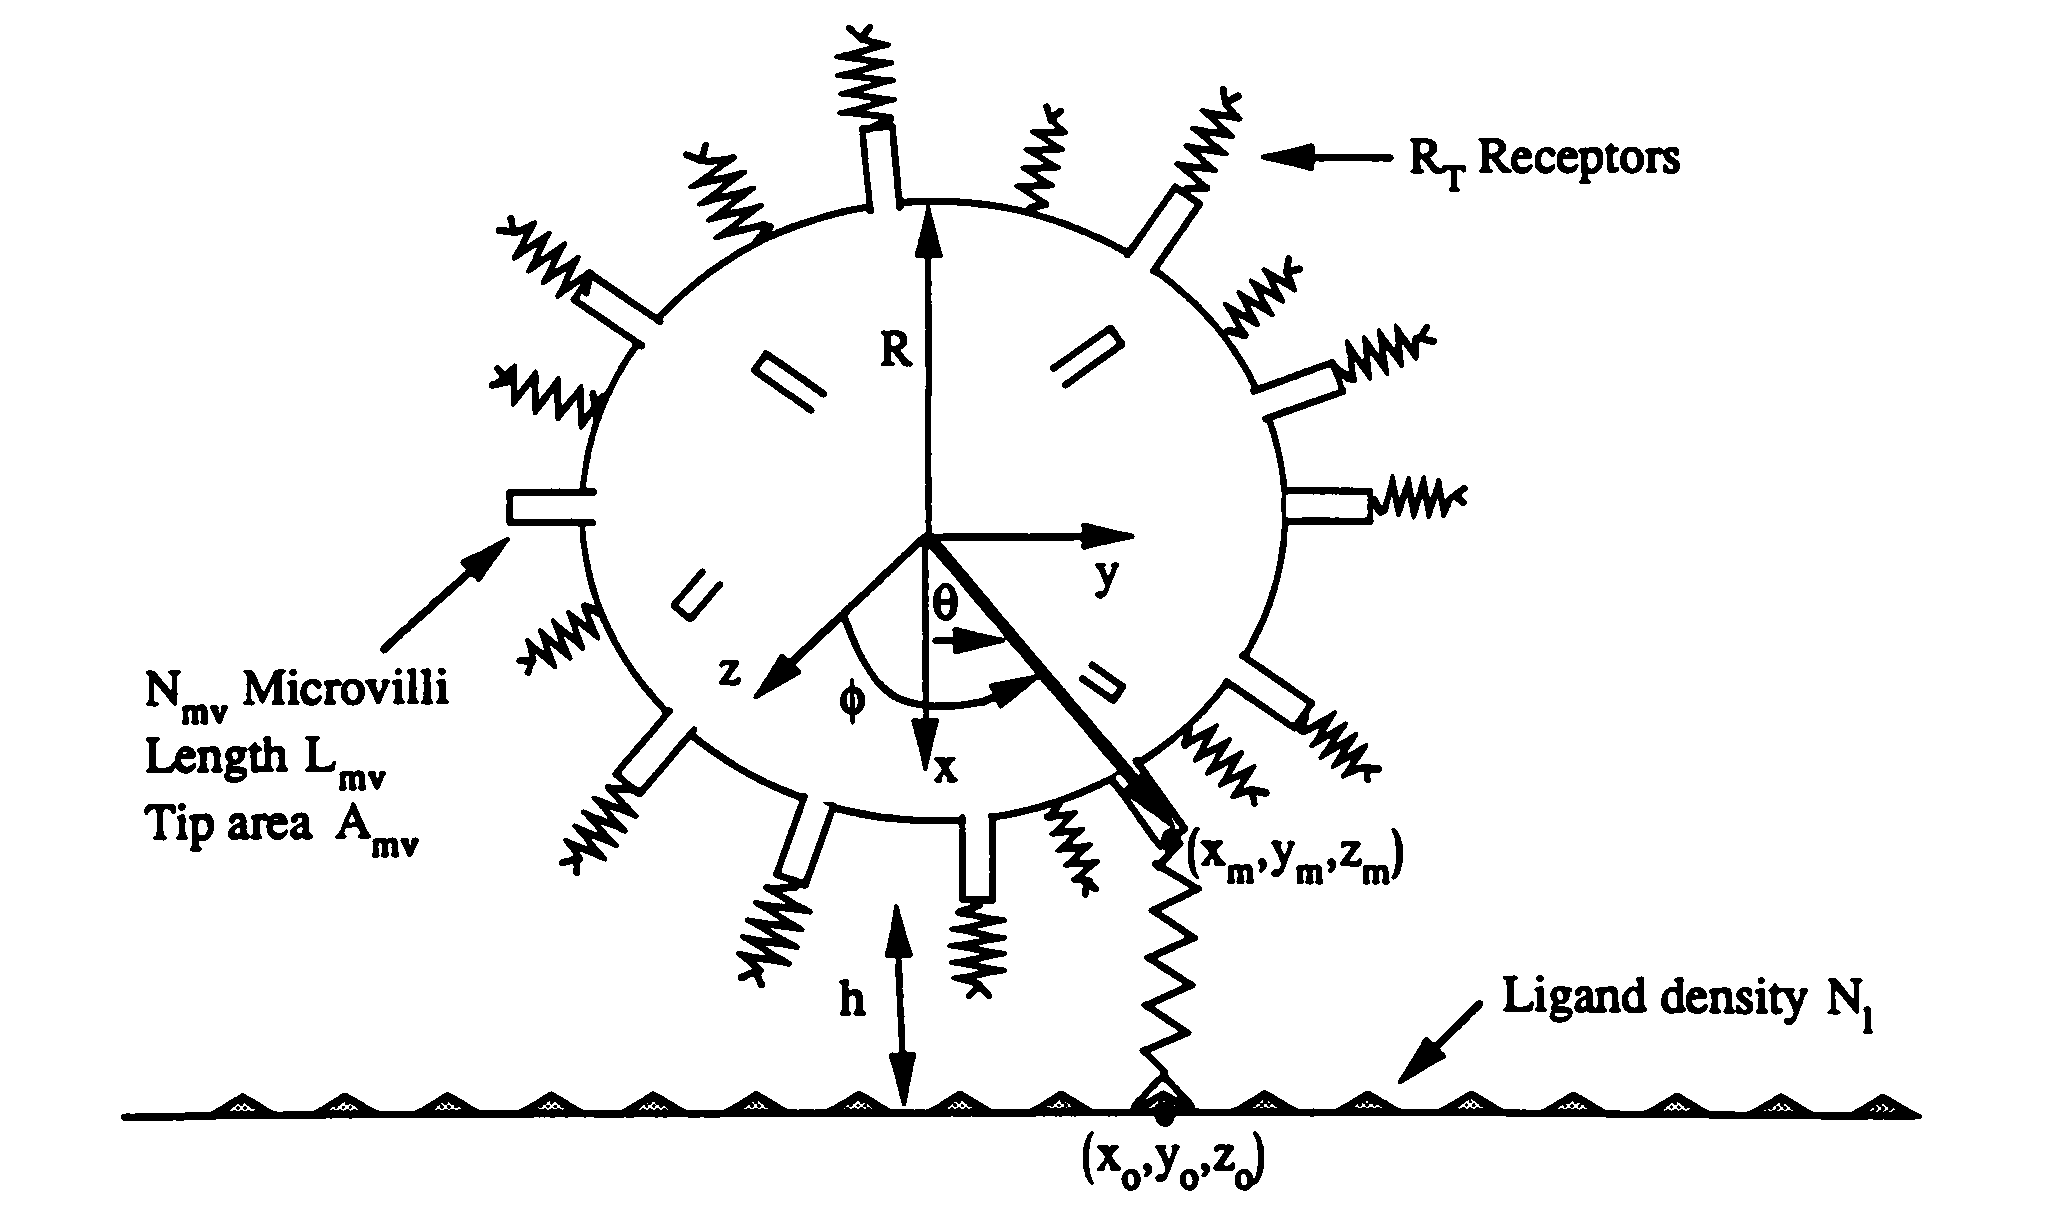
\includegraphics[width=\textwidth]{hammer92scr}}
      \caption{Geometry of a leukocyte AD model. From Hammer \&
        Apte, 1992}
      \label{fig:hammer-diagram}
    \end{figure}
  \end{column}
\end{columns}
\note[item] {We want to find parameters that give realistic rolling
  behavior in the 3D model, and tweak binding parameters to model the
  effects of priming on rolling behavior}
\end{frame}

\section{Numerics \& Model}

\begin{frame}{Definitions and domain}
  \begin{columns}
    \begin{column}{.5\textwidth}
      \begin{itemize}
      \item Fluid domain is the upper half space where $x > 0$
      \item Wall is the plane at $x = 0$
      \item Background flow: $\vect{v}^\infty = \gamma x \vect{e}_z$
      \item Platelet: ellipsoid with axes $1.5 \times 1.5 \times 0.5$,
        center of mass at $\vect{x}_c$, orientation vector
        $\vect{e}_m$
        \note[item] {$\vect{e}_m$ is a unit vector in the direction of
          the minor axis. This is sufficient to define the
          orientation, since the platelet is rotationally symmetric
          about the minor axis} 
      \item Fluid satisfies steady Stokes equations with no-slip BCs
        on the wall and platelet surface:
        \begin{align*}
          &\Delta \vect{v} = \nabla P, \, \nabla \cdot
            \vect{v} = 0 \\
          &\vect{v}(\vect{x})|_{\partial P} = \vect{U} +
            \vect{\Omega} \times \vect{x} \\
          &\vect{v}|_{x = 0} = 0, \, \vect{v}(\vect{x})|_{\|\vect{x}\|
            \rightarrow \infty} \rightarrow \vect{v}^\infty(\vect{x}) 
        \end{align*}
        \note[item] {$\vect{U}$ is the translational velocity of the
          platelet, and $\vect{\Omega}$ is the angular velocity of the
          platelet. Next, talk about platelet motion.}
      \end{itemize}
    \end{column}

    \begin{column}{.4\textwidth}
      \begin{figure}
        \centering
        \subfloat{\fbox{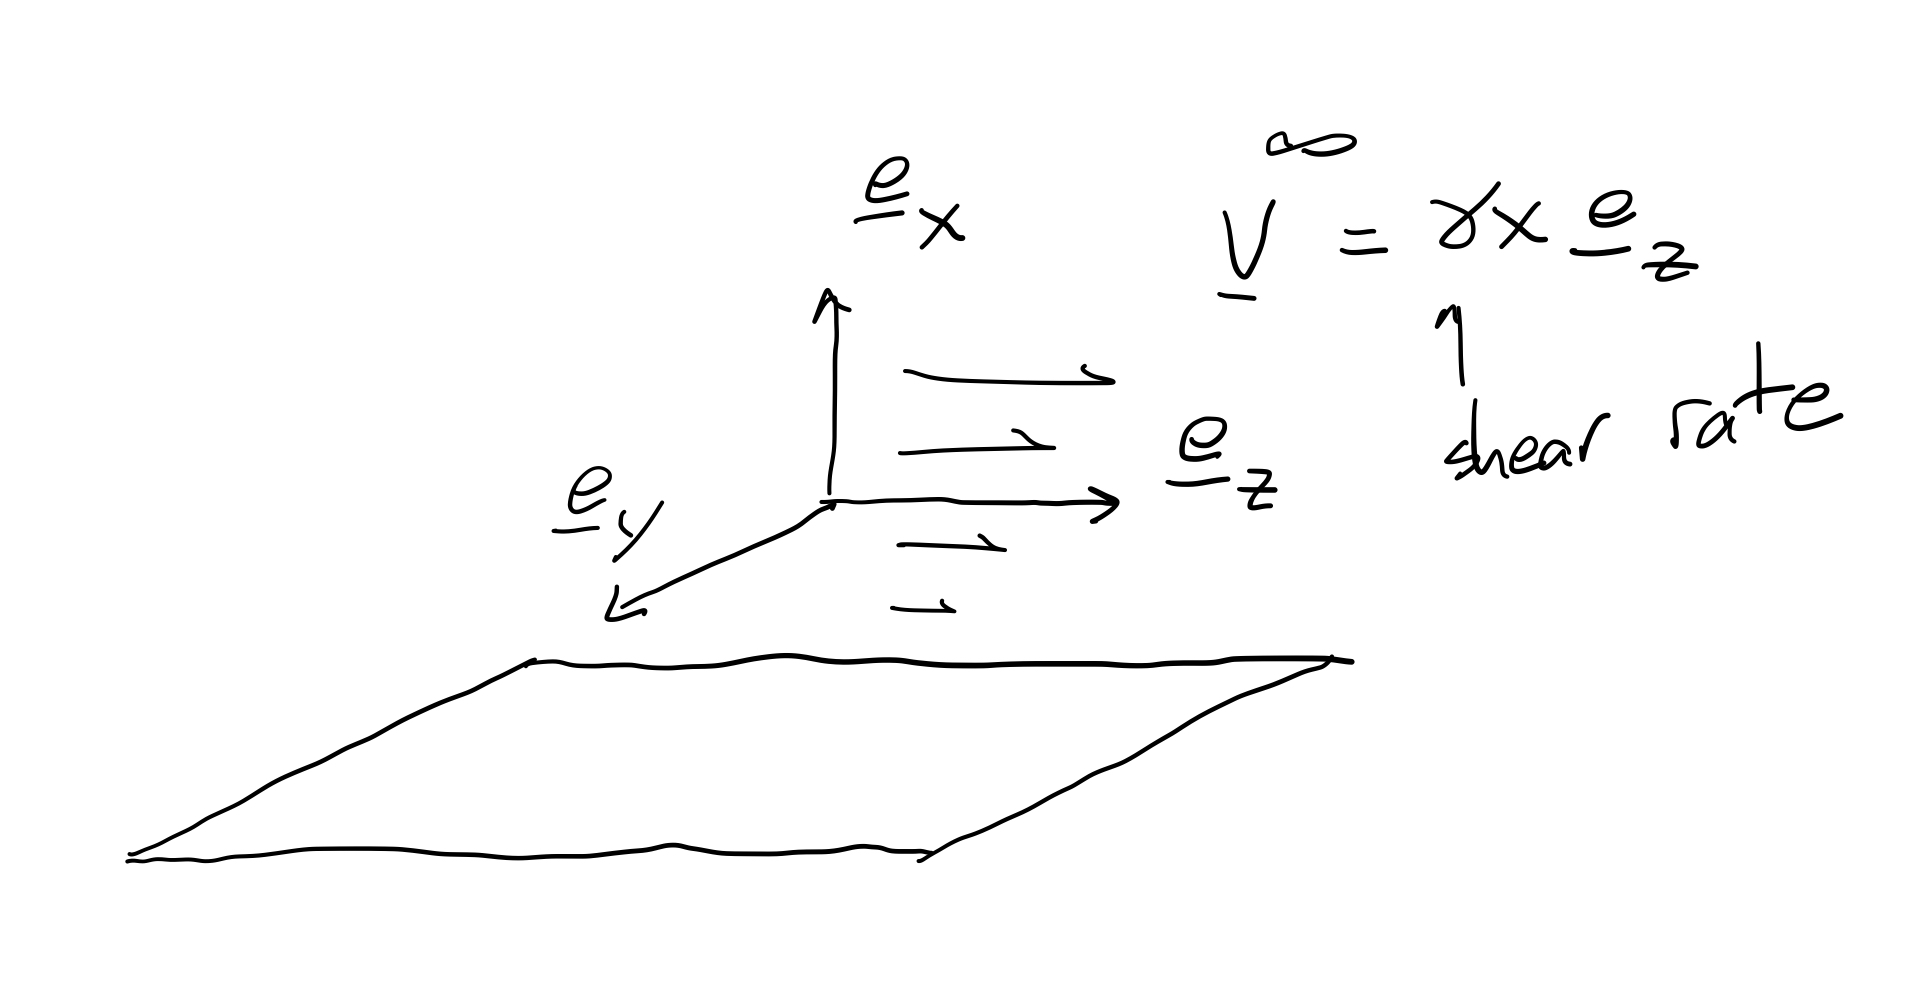
\includegraphics[width=\textwidth]{axes}}} \\
        \subfloat{\fbox{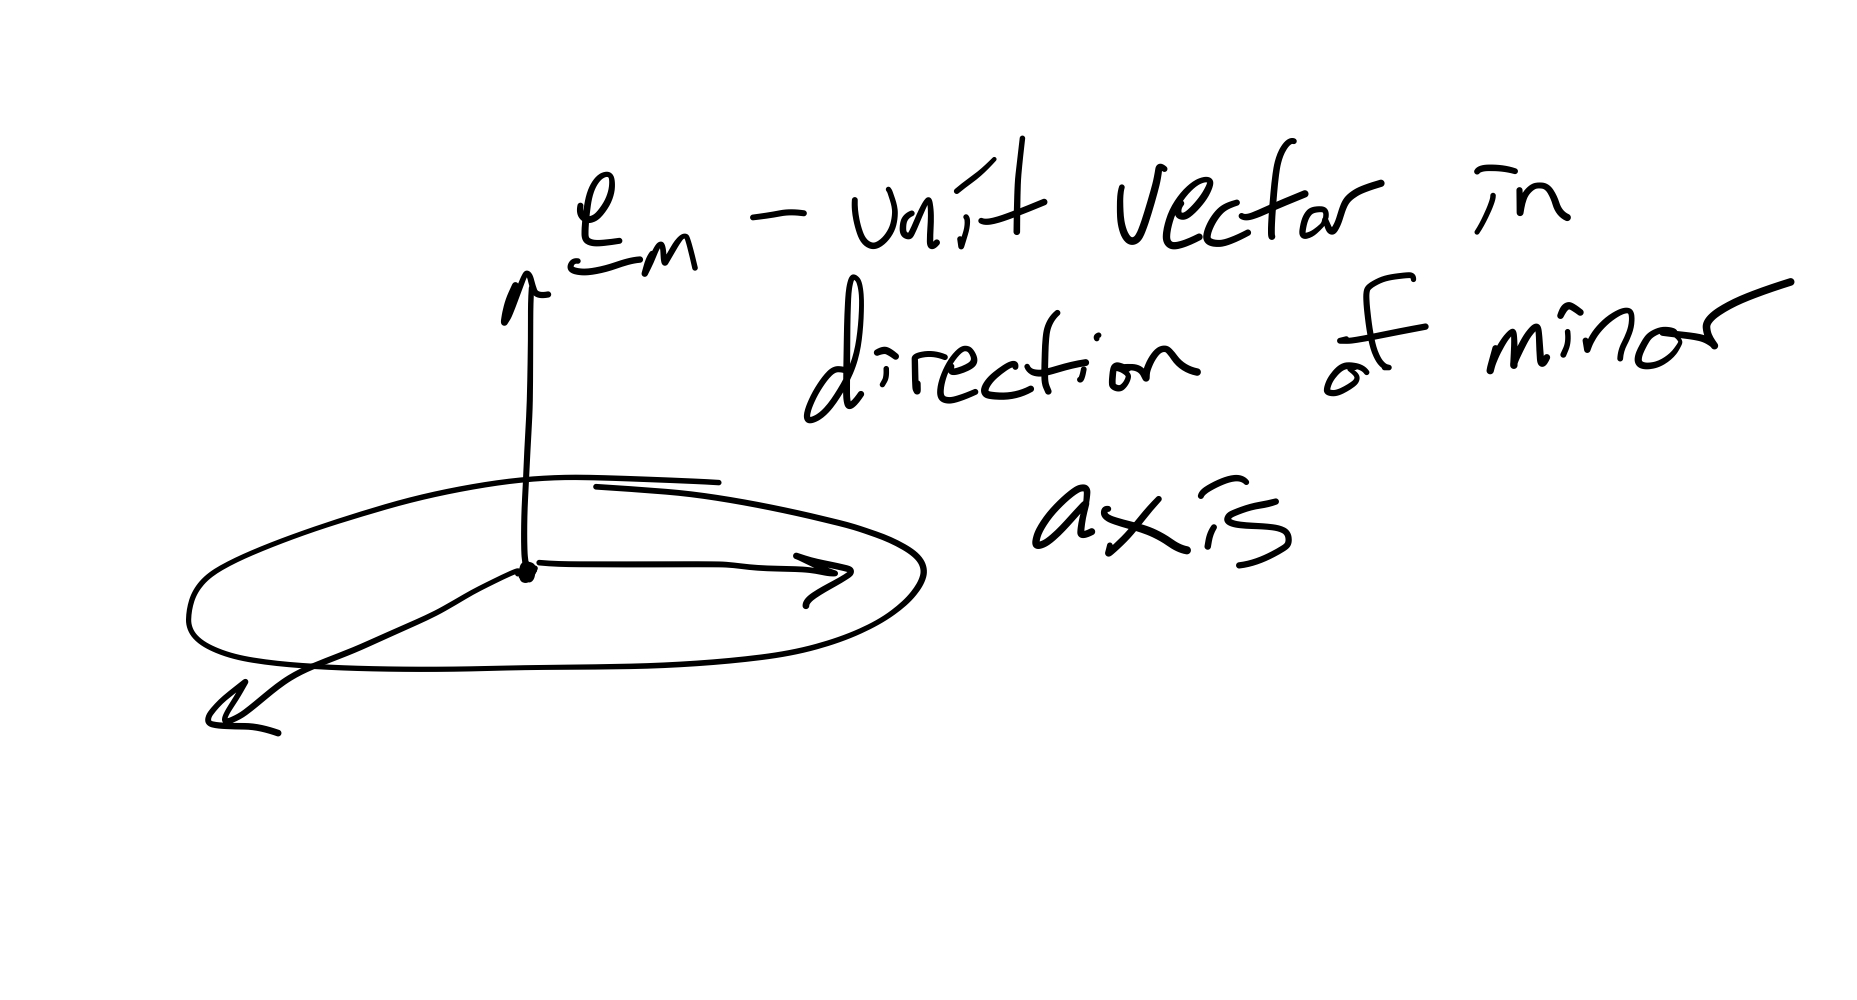
\includegraphics[width=\textwidth]{reference}}} 
        \caption{Sketch of the axes and orientation of the ellipsoid}
        \label{fig:orient-sketch}
      \end{figure}
    \end{column}
  \end{columns}
\end{frame}

\begin{frame}{Platelet motion}
  \begin{itemize}
    \note[item] {Equations of rigid body motion}
  \item Equations of motion:
    \begin{equation*}
      \frac{d\vect{x}_c}{dt} = \vect{U}(\vect{x}_c, \vect{e}_m), \,
      \frac{d\vect{e}_m}{dt} = \vect{\Omega}(\vect{x}_c, \vect{e}_m)
      \times \vect{e}_m
    \end{equation*}
    \note[item] {Of course, evaluating the RHS is the hard part}
  \item $\vect{U}$ and $\vect{\Omega}$ are found by balancing forces
    and torques on the platelet body.
  \item Define $\vect{F}^h$ and $\vect{T}^h$ to be the hydrodynamic
    forces on the platelet, and $\vect{F}^o$ and $\vect{T}^o$ to be
    other forces/torques acting on the platelet
    \note[item] {Most significantly bond forces, however past adhesive
      dynamics simulations have included other chemical forces acting
      on the platelet as well.}
  \item Given a velocity field $\vect{v}$, then
    \begin{align*}
      \vect{F}^h &= \int_{\partial P} \underline{\underline{\sigma}}
                   \cdot \vect{n} ds(\vect{x}) \\
      \vect{T}^h &= \int_{\partial P} (\vect{x} - \vect{x}_c) \times
                   \underline{\underline{\sigma}} \cdot \vect{n}
                   ds(\vect{x}) 
    \end{align*}
    \note[item] {$\sigma$ is the stress tensor of $\vect{v}$}
  \item If we assume $\vect{F}^o$ and $\vect{T}^o$ are known given a
    position and orientation, then we ``just'' need to find $\vect{U}$
    and $\vect{\Omega}$ such that $\vect{F}^h + \vect{F}^o = 0$
    \note[item] {This is hard because we need $\vect{U}$ and
      $\vect{\Omega}$ to solve Stokes' equations, but these are
      unknown at the start of a time step.}
  \end{itemize}
\end{frame}

\begin{frame}{Solving for $\vect{U}$ and $\vect{\Omega}$}
  \begin{itemize}
  \item We can decompose $\vect{F}^h$ into a drag force $\vect{F}^d$
    generated by a platelet moving through a stationary background
    flow, and $\vect{F}^s$ which represents the drag force on a
    stationary platelet in a background shear flow
    \note[item] {And same for the torques}
  \item Because of the linearity of Stokes flow, there is a linear
    relationship between $(\vect{F}^d, \vect{T}^d)$ and $(\vect{U},
    \vect{\Omega})$: 
    \begin{align*}
      \vect{F}^d &= -(\mathcal{T} \vect{U} + \mathcal{P}
      \vect{\Omega}) \\
      \vect{T}^d &= -(\mathcal{P}^T \vect{U} + \mathcal{R}
      \vect{\Omega}) 
    \end{align*}
  \item The resistance matrices $\mathcal{T}$, $\mathcal{P}$, and
    $\mathcal{R}$ depend only on the shape of the body, and its
    position and orientation
  \item The resistance matrices can be found by solving 6 different
    Stokes flow problems---three translations and three
    rotations
  \item $\vect{F}^s$ and $\vect{T}^s$ are found with 7th solve, where
    the platelet is stationary and the background flow is a shear flow
    \note[item] {These solves are done with regularized Stokeslets}
  \end{itemize}
\end{frame}

\begin{frame}{Regularized Stokeslets}
  \note[item] {I think I've already exceeded the number of math slides
    acceptable in this presentation}
  \begin{itemize}
  \item In the method of regularized Stokeslets, approximate point
    forces are placed on a structure (a surface, thin filament, or
    even discrete points)
  \item Analytic representations of fluid flow have been derived for
    these approximate point forces, and can be summed together to find
    the resulting fluid flow
  \item Often (and in my case), there is a desired \emph{velocity} at
    certain points, and the Stokeslets strengths must be solved for
  \end{itemize}
\end{frame}

\begin{frame}{Binding and Unbinding}
  \begin{itemize}
  \item One simple model of length dependent binding and unbinding
    comes from Dembo et. al. (1988):
    \begin{align*}
      k_f(r) &= k_f^0 \exp \left(\frac{-\sigma_\tn{ts} (r -
               \lambda)^2}{2k_B T} \right) \\
      k_d(r) &= k_d^0 \exp \left(\frac{(\sigma - \sigma_\tn{ts})(r -
               \lambda)^2}{2k_B T} \right) \\
    \end{align*}
    where $r = \| \vect{x}_\tn{receptor} - \vect{x}_\tn{ligand}
    \|$, $\lambda$ is the rest length of the receptor-ligand bond, and
    $\sigma$ and $\sigma_\tn{ts}$ are Hookean spring constants
  \item If $\sigma < \sigma_\tn{ts}$, then the bonds are slip bonds
  \item Some later AD models use catch-slip bond kinetics, which
    requires a more complicated model of binding and unbinding
    \note[item] {Receptors distributed uniformly over the surface of
      the platelet, and ligands distributed on the wall}
  \item From these rates, we can find probabilities of bonds
    forming/breaking within a time step
  \end{itemize}
\end{frame}

\begin{frame}{Current and Near-Future Work}
  \begin{itemize}
  \item I am working on adding stochastic binding and unbinding to the
    model
  \item Find parameter values that give reasonable rolling behavior
    \note[item] {These experiments are likely too expensive to do true
    parameter fitting; just want behavior that is close to observations}
  \item Run experiments with ``unprimed'' and ``primed'' (through
    changing binding parameters) platelets and assemble statistics
  \end{itemize}
\end{frame}

\end{document}
